\documentclass[aps,
%prl,
twocolumn,
showpacs,
superscriptaddress,groupedaddress]{revtex4}


\usepackage{amssymb}
\usepackage{amsmath}
\usepackage{float}
\usepackage{graphicx}
\usepackage[caption=false]{subfig}
\usepackage{subfig}
\usepackage{mathrsfs}

\newcommand{\dmcomment}[1]{{\tt #1}}

\begin{document}

\title{Theory of the crossover from lasing to steady state superradiance}
\author{D. A. Tieri}
\affiliation{JILA, University of Colorado, Boulder}
\author{Minghui Xu}
\affiliation{JILA, University of Colorado, Boulder}
\author{D. Meiser}
\affiliation{Tech-X Corporation, 5621 Arapahoe Avenue,
             Boulder, Colorado 80303, USA.}
\author{J. Cooper}
\affiliation{JILA, University of Colorado, Boulder}
\author{M. J. Holland}
\affiliation{JILA, University of Colorado, Boulder}
\date{\today}

\begin{abstract}
  Lasing and steady state superradiance are two phenomena that may
  appear at first glance to be distinct, but in fact should be thought
  of as the two extreme limits of a continuous crossover.  In a laser,
  phase information maintained by a macroscopic intracavity light field,
  and the robustness of this phase is what leads to the coherence
  properties of the output light.  In contrast, in steady-state
  superradiant systems, the coherence derives from the macroscopic
  collective dipole of a many-atom ensemble.  In this paper, we develop
  a quantum theory that connects smoothly between these two extreme
  limits.  The properties of systems that lie in the superradiance,
  lasing, and crossover parameter regions are contrasted and compared.
  We find that for a given output intensity a narrower linewidth can be
  obtained by operating closer to the superradiance side of the
  crossover.  We find that robustness against cavity frequency
  fluctuations can be greatly reduced in the superradiance limit.
  Brightness, narrow intrinsic linewidth, and robustness against
  perturbations make light sources based on steady state superradiance
  promising systems for ultra-stable local oscillators for precision
  measurement applications.
\end{abstract}

\pacs{42.50.Nn, 06.30.Ft, 37.30.+i, 42.50.Ct}


\maketitle

\section{Introduction}

Since its first demonstration in 1960~\cite{maiman1960stimulated}, the
laser has had a profound impact on fundamental science research and
numerous areas of society.  Lasers are integral to many fields of
research and technological applications, ranging from atomic and
molecular physics research, atomic clocks, the global positioning
system, nuclear fusion research, biology research, medicine, and
consumer electronics.  Although many different types of lasers exist,
with their characteristic parameters (such as intensity, power,
linewidth, physical size) spanning many orders of magnitude, all lasers
share a common conceptual foundation.  A laser is a cavity quantum
electrodynamics (QED) system consisting of a gain medium inside an
optical cavity.  We will oftentimes refer to the gain medium as
``atoms'' for brevity.  Lasers typically operate in the good cavity
regime of cavity QED where the linewidth of the cavity is much narrower
than the bandwidth of the gain medium.  The atoms generate a coherent
electromagnetic field in the cavity by means of stimulated
emission~\cite{PhysRev.112.1940}.  Stimulated emission is a quantum
mechanical interference effect in which the presence of a large number
of photons in a particular mode of a light field increases the
probability that an atom will emit into that mode. The energy emitted
into the cavity field has to be replenished by some repumping mechanism
to achieve steady state operation. In a laser, the macroscopic phase
information that is associated with the coherence of the generated
radiation is encoded in the light field.

Around the same time as the laser was first demonstrated, the effect
of superradiance was predicted~\cite{PhysRev.93.99}, and soon
thereafter, experimentally demonstrated.  Superradiance is a quantum
mechanical interference effect in which correlations between atoms
lead to collective emission.  Superradiance has most commonly been
considered as a pulsed phenomenon.  Atoms in an ensemble are prepared
in the excited state.  Spontaneous emission into one or a few spatial
modes is then enhanced via growth of atom-atom correlations.
However, it has been known for some time that superradiance can also
occur in steady state~\cite{PhysRevLett.102.163601,
  PhysRevA.81.033847, PhysRevA.81.063827,PhysRevLett.89.253003} by
placing the atomic ensemble inside a cavity.  In contrast to lasers,
superradiance in steady-state occurs in a cavity with a much broader
linewidth than the atomic linewidth.  This regime is referred to as
the bad-cavity limit of cavity QED~\cite{PhysRevA.51.809,
  PhysRevLett.72.3815, ChenDeliciousLaser, HakenLaser,
  HakenLaserBook}.  The radiation produced in steady state
superradiance is also coherent.  However, in contrast to a laser, the
coherence is encoded in the atomic medium.  Progress has recently been
made towards the experimental
verification~\cite{ThompsonPaper,bohnet2012relaxation} of this proposal.

An important application of lasers is as a stable local oscillator for
optical atomic clocks and precision spectroscopy.  These lasers rely on
stabilization against reference cavities.  The most advanced such lasers
reach linewidths of $< 0.1 {\rm Hz}$ corresponding to quality factors of
$Q>10^{15}$~\cite{Cole:TenfoldReductionBrownianNoise}. The principal
limiting factor in the way of further improvement of these local
oscillators is thermal vibrations of the dielectric coatings in the
cavity mirrors~\cite{PhysRevLett.101.260602}.  To overcome this
technical challenge, researchers have proposed an alternate approach
using an active system based on steady state superradiance on a clock
transition to create an even more stable light
source~\cite{PhysRevLett.102.163601, ChenDeliciousLaser}.  However, this
proposal has challenges of its own.  First of all, in spite of the
enhancement that occurs due to superradiance, the produced intensity is
orders of magnitude lower than for a conventional laser.  Second of all,
perturbations of atomic transition frequencies can potentially lead to
phase and frequency perturbations in the generated field.

In this paper we develop a unified theory for lasers and steady state
superradiance.  In this unified theory, lasers and steady state
superradiance are the extreme limits of a continuous crossover and the
theory continuously interpolates between the two.  This allows us to
directly compare and contrast lasers, steady state superradiant systems,
and systems in the crossover region using the same language.  Our
analysis thus further clarifies the qualitative and quantitative
differences between lasing and steady state superradiance.  From the
perspective of applications the unified theory enables us to determine
the optimal system for ultra stable local oscillators and precision
measurement applications.

We analyze the model using different levels of approximation: An exact
method using SU(4) operators, a semi-classical method based on {\it
c}-number Langevin equations, a quantum phase diffusion model for the
field amplitude, and a mean field model.  The different approaches provide insight into
different aspects of the problem.  Highly simplified models like the
mean field equations and phase diffusion yield a qualitative
understanding of the general characteristics of systems throughout the
crossover.  By comparison between the approximations we can
differentiate between truly critical physical effects and less important
details.  We find that fluctuations and correlations are essential for
the noise properties of the system (e.g. the linewidth of the generated
light) but that the fluctuations and correlations can be modelled
semi-classically.  Comparison with the exact SU(4) method for small
numbers of atoms shows that {\it c}-number Langevin equations provide an
accurate description of the system.  Due to their much smaller
computational complexity, we are then able to use the {\it c}-number
Langevin equations to quantitatively study much larger systems relevant
for experiment.

The rest of this paper is organized as follows.  In
section~\ref{sec:Model} we summarize the physical model upon which our
analysis is based. In \ref{sec:Methods} we discuss several approximation
methods.  We compare the approximations with one another to determine
their accuracy and to evaluate their ability to capture the various
physical signatures. In section \ref{sec:CrossoverCharacterization} we
define a crossover parameter which characterizes the relative importance
of stimulated emission to collective atomic effects in a cavity QED
system.  In section~\ref{sec:Results} we discuss our results on the
crossover.


\section{Model}
\label{sec:Model}

As noted in the introduction, the fundamental ingredients of lasers and
superradiance systems are an electromagnetic field and atoms serving as
a gain medium.  A minimal model consists of a single mode cavity field
and an ensemble of two level atoms.  The atoms couple to the
cavity field via the dipole interaction.  Energy is supplied to the
system by means of a continuous repumping mechanisms that transfers
atoms from the ground state to the excited state.  In practice, this
optical pumping necessitates a third atomic level.  But we assume that
atoms quickly decay from that third level to the atomic excited state
allowing the third level to be eliminated from the model.  The
repumping and atomic and cavity relaxation processes make the system an
open quantum system.

Mathematically, our model is described by the quantum Born-Markov master
equation,
\begin{equation}
  \frac{d}{dt} \hat{\rho} =
  \frac{1}{i \hbar} \left[ \hat{H}, \hat{\rho} \right] +
  \hat{\mathcal{L}}\left[ \hat{\rho} \right],
\label{ME1Crossover}
\end{equation}
where,
\begin{equation}
\hat{H} = \frac{\hbar \omega_a}{2} \sum_{j=1}^{N} \hat{\sigma}^{z}_{j}
+ \hbar \omega_c \hat{a}^{\dagger}\hat{a}
+ \frac{\hbar \Omega}{2}  \sum_{j=1}^{N} \left(
    \hat{a}^{\dagger} \hat{\sigma}^{-}_{j} +
    \hat{\sigma}^{+}_{j} \hat{a} \right)\;.
\end{equation}
The Liouvillian superoperator $\hat{\mathcal{L}}\left[ \hat{\rho}
\right]$ describes the various decay and noise processes as well as the
repumping.

The Hamiltonian $\hat{H}$ describes the coherent evolution of the
coupled atom cavity system, where $\omega_{a}$ is the atomic transition
frequency and $\omega_c$ is the frequency of the cavity mode. The Pauli
spin matrices for the atoms are $\hat{\sigma}_j^{+}$,
$\hat{\sigma}_j^{-}$ and $\hat{\sigma}_j^{z}$, and $\hat{a}$ is the
annihilation operator of the cavity mode. The atom-cavity coupling rate
is $\Omega$.  In general, the atom-cavity coupling depends on the
location of the atom in the cavity field.  To simplify the discussion, we ignore
such spatial effects because they are known to result in only minor
quantitative changes.  In principle, a constant $\Omega$ could be
realized experimentally by confining the atoms to locations of equal
amplitude of the cavity mode by means of an optical lattice.

The incoherent evolution is described by the Liouvillian
$\hat{\mathcal{L}}\left[ \hat{\rho} \right]$,
\begin{eqnarray}
\hat{\mathcal{L}}\left[ \hat{\rho} \right] &=&
  -\frac{\kappa}{2}
  \left(
    \hat{a}^{\dagger} \hat{a} \hat{\rho}
    + \hat{\rho}  \hat{a}^{\dagger} \hat{a}
    - 2\hat{a} \hat{\rho} \hat{a}^{\dagger}
  \right)
\nonumber
\\
 &&-\frac{\gamma}{2} \sum_{j=1}^N
  \left(
   \hat{\sigma}_{j}^{+} \hat{\sigma}_{j}^{-} \hat{\rho}
   + \hat{\rho} \hat{\sigma}_{j}^{+} \hat{\sigma}_{j}^{-}
   - 2\hat{\sigma}_{j}^{-} \hat{\rho} \hat{\sigma}_{j}^{+}
  \right)
\nonumber
\\
 &&-\frac{w}{2} \sum_{j=1}^N
  \left(
   \hat{\sigma}_{j}^{-} \hat{\sigma}_{j}^{+} \hat{\rho}
   + \hat{\rho} \hat{\sigma}_{j}^{-} \hat{\sigma}_{j}^{+}
   - 2\hat{\sigma}_{j}^{+} \hat{\rho}  \hat{\sigma}_{j}^{-}
  \right),
\nonumber
\\
 &&+\frac{1}{2T_2} \sum_{j=1}^N
  \left(
   \hat{\sigma}_{j}^{z} \hat{\rho}  \hat{\sigma}_{j}^{z} - \hat{\rho}
  \right),
\end{eqnarray}
where $\hat{\rho}$ is the system's density matrix, $\kappa$ is the decay
rate of the cavity, $\gamma$ is the natural decay rate of the atoms, $w$
is the repumping rate, and $\frac{1}{T_2}$ is the inhomogeneous
dephasing rate.


\section{Solution Methods}
\label{sec:Methods}

Direct numerical solution of Eq.~(\ref{ME1Crossover}) is impossible for
experimentally relevant numbers of particles because the dimension of
the Hilbert space of the system scales as $2^N$.  In this section we
introduce several solution methods and approximations to overcome the
exponential scaling of the size of the Hilbert space.  They can be
grouped into three categories: Exact methods (SU(4) method with
Monte-Carlo simulation); semi-classical methods ({\it c}-number Langevin
equations, phase diffusion); and mean field
treatment.  The exact solution methods solve the quantum mechanical
problem directly without further approximations.  But of course they are
only practical for small numbers of atoms.  Semi-classical methods aim
to capture the physics of the system correctly for large $N$.  They
include a classical representation of noise, fluctuations, and
correlations.  Comparison with direct solution methods for small $N$
allows us to verify the validity and accuracy of the semi-classical
approach.  Finally, the mean field method neglect fluctuations to arrive
at simple equations for mean values.  The mean field equations admit
closed form solutions that provide valuable qualitative insights.

The SU(4) method provides a direct numerical solution of
Eq.~(\ref{ME1Crossover}) by exploiting an underlying permutation
symmetry to drastically reduce the Hilbert space
dimension~\cite{Hartmann:arXiv1201.1732, PhysRevA.87.062101}.  The
resulting master equation is solved using the quantum jump
method~\cite{Dalibard92,Dum92,Knight98}.  Details of the method have
been described previously in~\cite{PhysRevA.87.062101} and we summarize
the main results in Appendix~\ref{Su4Appendix} to make this paper self
contained.

\if 0
Even with the ability to describe problems with larger photon number, the SU(4) method can only describe systems much smaller than many realistic experimental situations. We therefore must introduce approximations in order to handle these larger systems.

The {\it c}-number Langevin method \cite{Scully97, PhysRevA.47.1431} approximates the quantum
Langevin equations which are equivalent to Eq.~(\ref{ME1Crossover}) as complex variable equations with Gaussian fluctuations.
These equations do not scale with $N$ in the same way, and therefore can often be used to treat systems with large $N$ where an exact treatment is not possible. 

When the additional approximation is added that the system only exhibits phase diffusion, {\em i.e.}\ amplitude fluctuations are neglected, an analytic solution for the linewidth of the power spectrum can be obtained \cite{HakenLaser, HakenLaserBook}. This method is described in Appendix~\ref{HakenAppendix}.
Finally, the mean field solutions of the quantum Langevin equations, neglect all fluctuations. These solutions 
can not be used to describe the linewidth, but prove useful for other system observables.

\fi

\subsection{Quantum Langevin Equations}

For the derivation of the semi-classical equations corresponding to 
Eq.~(\ref{ME1Crossover}) it is more convenient to go over to the
Heisenberg picture.  The resulting equations are the quantum Langevin
equations
\begin{equation}
\frac{d}{dt} \hat{a}= -\frac{1}{2} (\kappa +2i\omega_c) \hat{a}
-\frac{i N \Omega}{2} \hat{S}^{-}
+\hat{F}^{a},
\label{La}
\end{equation}
\begin{equation}
\frac{d}{dt} \hat{S}^{-} =
-\frac{1}{2} \left(\Gamma +2 i \omega_a \right)  \hat{S}^{-}
+\frac{i \Omega}{2} \hat{a} \hat{S}^{z}
+\hat{F}^{-},
\label{Lsm}
\end{equation}
\begin{equation}
\frac{d}{dt} \hat{S}^{z} =
-(w+\gamma)\left( \hat{S}^{z} - d_0\right)
+i\Omega \left( \hat{a}^{\dagger}\hat{S}^{-} -
\hat{a}\hat{S}^{+} \right)
+\hat{F}^{z},
\label{Lsz}
\end{equation}
where $\delta=\omega_{a}-\omega_{c}$. We have defined the collective
operators,
\begin{eqnarray}
\hat{S}^{-}&=&\frac{1}{N}\sum_{k=1}^N \hat{\sigma}_k^{-},
\nonumber
\\
\hat{S}^{z}&=&\frac{1}{N}\sum_{k=1}^N \hat{\sigma}_k^{z},
\nonumber
\end{eqnarray}
where $\Gamma \equiv w+\gamma+\frac{2}{T_2}$, $d_0 =
\frac{w-\gamma}{w+\gamma}$ and where $\hat{S}^{+}$ and $\hat{S}^{-}$ are
Hermitian conjugates of one another, $\hat{S}^{+} =
(\hat{S}^{-})^{\dagger}$. The noise operators $\hat F^\mu$ have zero
mean and their second order correlations are given by
\begin{equation}
\left< \hat{F}^{\mu}(t) \hat{F}^{\nu}(t^{\prime})\right> =
2 D^{\mu \nu} \delta(t-t^{\prime})\;.
\end{equation}
The diffusion matrix elements $D^{\mu \nu} $ can be calculated using the
Einstein relations \cite{meystre2007elements},
\begin{eqnarray}
&& 2D^{a a^{\dagger}}= \kappa \nonumber \\
&& 2D^{+-}= \frac{1}{N}
\left(
  w + \frac{1}{T_2} \left(1 + \left< \hat{S}^{z} \right> \right)
\right) \nonumber \\
&& 2D^{-+}= \frac{1}{N}
\left(
  \gamma + \frac{1}{T_2} \left(1- \left< \hat{S}^{z} \right> \right)
\right) \nonumber \\
&& 2D^{+z}= -\frac{2w}{N} \left< \hat{S}^{+} \right>
\hspace{0.83in} 2D^{z+}= \frac{2\gamma}{N} \left< \hat{S}^{+} \right>
\nonumber \\
&& 2D^{-z}= \frac{2\gamma}{N} \left< \hat{S}^{-} \right>
\hspace{0.86in} 2D^{z-}= -\frac{2w}{N} \left< \hat{S}^{-} \right>
\nonumber \\
&& 2D^{zz}= \frac{2\gamma}{N}
\left(1+ \left< \hat{S}^{z} \right> \right) +
\frac{2w}{N}\left(1- \left< \hat{S}^{z} \right> \right).
\label{OpNoise1}
\end{eqnarray}


\subsection{{\it c}-number Langevin equations for numerical simulations}

The quantum Langevin equation are operator valued stochastic
differential equations.  As such they are not suited for practical
computations.  To obtain practical equations we construct a
semi-classical theory by replacing the operators in the quantum Langevin
equations by {\it c}-numbers,
\begin{equation}
\frac{d}{dt} a= -\frac{1}{2}  (\kappa +2i\omega_c) a
-\frac{i N \Omega}{2} S^{-}
+F^{a},
\label{Lac}
\end{equation}
\begin{equation}
\frac{d}{dt} S^{-} = -\frac{1}{2}  \left(\Gamma +2 i \omega_a \right)  S^{-}
+\frac{i \Omega}{2} a S^{z}
+F^{-},
\end{equation}
\begin{equation}
\frac{d}{dt} S^{z} = -(w+\gamma)\left( S^{z} - d_0\right)
+i\Omega \left( a^{\dagger}S^{-} - a S^{+} \right)
\label{Lszc}
+F^{z},
\end{equation}
where the omission of the hats over the variables signifies that they
are {\it c}-numbers.  The noise terms $F^a$, $F^-$, and $F^z$ should be
interpreted according to the rules of Ito calculus.  The noises are
correlated according to
\begin{equation}
\left< F^{\mu}(t) F^{\nu}(t^{\prime})\right> =
2 \mathscr{D}^{\mu \nu} \delta(t-t^{\prime})\;.
\label{ClassicalDiffusion1}
\end{equation}

It is easier to construct the semi-classical equations by introducing
real variables according to
\begin{eqnarray}
\hspace{-0.5in} \hat{q} &=&
\frac{1}{2} \left( \hat{a}^{\dagger} + \hat{a} \right),
\hspace{0.48in} \hat{p} =
\frac{1}{2i} \left( \hat{a}^{\dagger} - \hat{a} \right),
\\
\hat{S}^x &=&
\frac{1}{2} \left( \hat{S}^{+} + \hat{S}^{-} \right),
\hspace{0.2in} \hat{S}^y =
\frac{1}{2i} \left( \hat{S}^{+} - \hat{S}^{-} \right)\;.
\end{eqnarray}
The equations of motion in terms of these variables are
\begin{eqnarray}
\frac{d}{dt} q &=& -\kappa q - 2 \omega_c p - N \Omega S^{y} + F^{q},
\label{cq1}
\\
\frac{d}{dt} p&=& -\kappa p + 2 \omega_c q + N \Omega S^{x} + F^{p},
\\
\frac{d}{dt} S^{x} &=&
-\Gamma S^{x}  - 2 \omega_a S^{y} + \Omega p S^{z} + F^{x},
\\
\frac{d}{dt} S^{y} &=&
-\Gamma S^{y}  + 2 \omega_a S^{x} - \Omega q S^{z} + F^{y},
\\
\frac{d}{dt} S^{z} &=& -(w+\gamma)\left( S^{z} - d_0\right)
+2 \Omega \left( q S^{y} - p S^{x} \right)
+F^{z}\;.
\nonumber
\\
\label{eqn:cnumberlangevin}
\end{eqnarray}

The correspondence between the semi-classical and quantum mechanical
Langevin equations is established by requiring that they produce
identical equations for first and second moments of the system
operators.  Comparison of the first moments (i.e. the expectation
values of the equations of motion) leads to
\begin{equation}
\langle F^q\rangle = 
\langle F^p\rangle = 
\langle F^x\rangle = 
\langle F^y\rangle = 
\langle F^z\rangle = 0\;,
\end{equation}

Comparison of the second moments allows us to find the classical
diffusion matrix elements $\mathscr{D}^{\mu \nu}$ from the quantum
mechanical ones.  To make this procedure well defined we have to choose
a specific ordering of the quantum mechanical operators.  We choose to
make the correspondence using symmetric ordering defined by the
symmetric expectation value
\begin{equation}
\left< \hat{A}^{\mu} \hat{A}^{\nu} \right>_s=
\frac{1}{2} \left( \left< \hat{A}^{\mu} \hat{A}^{\nu} \right> + \left<
\hat{A}^{\nu} \hat{A}^{\mu} \right> \right)\;,
\end{equation}
where $\hat{A}^{\mu}$ and $\hat{A}^{\nu}$ are generic system operators.
We point out that in this formulation, the classical Langevin equations
are equivalent to a Fokker-Planck equation for the Wigner
quasi-probability distribution.  A tedious but straightforward
calculation yields
\begin{eqnarray}
&& 2\mathscr{D}^{q q}=
\frac{\kappa}{4} \hspace{0.7in} 2\mathscr{D}^{p p}=
\frac{\kappa}{4} \nonumber \\
&& 2\mathscr{D}^{xx}=
\frac{\Gamma}{4N} \hspace{0.57in} 2\mathscr{D}^{yy}=
\frac{\Gamma}{4N} \nonumber \\
&& 2\mathscr{D}^{xz}=
2\mathscr{D}^{zx}=
\frac{-w+\gamma}{N} \left< \hat{S}^{x} \right>  \nonumber \\
&& 2\mathscr{D}^{yz}=
2\mathscr{D}^{zy}=
\frac{-w+\gamma}{N} \left< \hat{S}^{y} \right>  \nonumber \\
&& 2\mathscr{D}^{zz}=
\frac{2}{N}\left((w+\gamma) + (-w+\gamma)  \left< \hat{S}^{z} \right> \right).
\label{cNoise1}
\end{eqnarray}

We solve the stochastic differential equations
(\ref{eqn:cnumberlangevin}) by means of the explicit second order weak scheme \cite{kloeden2011numerical}. An ensemble of trajectories can be evolved simultaneously and the expectation values appearing in Eq.~(\ref{cNoise1}) can be calculated from the ensemble. This allows the additive form of the explicit second order weak scheme to be used, which is simpler than the general form.

The noises $F^\mu$ are found by means of
\begin{equation}
F^\mu=\sum_\nu \sqrt{\lambda_\nu} M_{\mu,\nu}^T f^\nu\;,
\end{equation}
where $M_{\mu,\nu}$ is the orthogonal matrix that
diagonalizes the diffusion matrix, $\lambda_\nu$ are its eigenvalues,
and $f^\nu$ are independent normalized Wiener processes.
It was found empirically that the symmetrically ordered diffusion matrix is positive definite when the system is above the first threshold (defined in Sec.~(\ref{MFE})). Below this threshold, the symmetrically ordered diffusion matrix is not positive definite, and divergent trajectories can occur. Typically, an ensemble of 1000 trajectories can be used to achieve convergence to within a few percent.


\subsection{Mean Field Equations}
\label{MFE}

By taking expectation values of the semi-classical
Eqns.~(\ref{cq1})--(\ref{eqn:cnumberlangevin}) we obtain the so called
mean field equations

\begin{equation}
\frac{d}{dt} a_0= -\frac{1}{2} (\kappa +2i(\omega_c-\omega)) a_0
-\frac{i N \Omega}{2} S_0^{-},
\label{La0}
\end{equation}
\begin{equation}
\frac{d}{dt} S_0^{-} =
-\frac{1}{2} \left(\Gamma +2 i (\omega_a-\omega) \right)  S_0^{-}
+\frac{i \Omega}{2} \hat{a} S_0^{z},
\end{equation}
\begin{equation}
\frac{d}{dt} S_0^{z} = -(w+\gamma)\left( S_0^{z} - d_0\right)
+i\Omega \left( a_0^{\dagger} S_0^{-} - a_0 S_0^{+} \right)\;.
\label{Lsz0}
\end{equation}
The noise terms drop out because they have zero mean.  The mean field
equations capture many of the most important features of the physical
system because the noise terms scale as $\sqrt{N}$ while the
expectation values scale as~$N$.  In the limit of large numbers of
atoms the noise terms are therefore less important.  Note that
Eqns.~(\ref{La0})--(\ref{Lsz0}) are written in the reference frame
rotating at frequency $\omega$.

Eqns.~(\ref{La0})--(\ref{Lsz0}) can be written in steady-state by
setting the left hand sides to zero and then solved in closed form.
We find
\begin{equation}
S_0^{z}=
\frac{(\kappa+2i(\omega_c-\omega))(\Gamma+2i(\omega_a-\omega))}{N\Omega^2}
\label{Sz01}
\end{equation}
for the steady state inversion. From this, the oscillation frequency
of the atom-cavity coupled system $w$ can be determined using the
condition that $S_0^{z}$ must be real, giving
\begin{equation}
\omega = \frac{\kappa \omega_a + \Gamma \omega_c}{\kappa+\Gamma}\;.
\label{atomcavityfrequencycenter1}
\end{equation}
When $\delta = \omega_a-\omega_c \ll \Gamma,\kappa$ the inversion can be
simplified to
\begin{equation}
S_0^{z}\approx \frac{1}{\mathcal{C}}\;,
\end{equation}
where $\mathcal{C}\equiv \frac{N \Omega^2}{\kappa \Gamma}$ is the
generalized many-atom cooperativity parameter (generalized since here
the effective linewidth $\Gamma$ includes the incoherent repumping $w$
as well as the single atom linewidth $\gamma$ and dephasing $1/T_2$).

In the same limit of small detuning we find for the steady state photon
number
\begin{equation}
|a_0|^2=\frac{N(w+\gamma)}{2 \kappa} (d_0 - \frac{1}{\mathcal{C}})\;.
\label{a0sqSS}
\end{equation}
The photon number has a maximum at
\begin{equation}
w=w_{\mathrm{opt}} = \frac{N \Omega^2}{2\kappa} - \gamma - \frac{1}{T_2}.
\label{wopt}
\end{equation}
In the limit where the collective decay rate $\mathcal{C}\Gamma$ is
much larger than the single atom rates $\gamma$ and $\frac{1}{T_2}$ we
find a simple expression for the maximum photon number,
\begin{equation}
(|a_0|^2)_{\mathrm{opt}}= \frac{N^2 \Omega^2}{8\kappa^2}\;.
\label{adaopt}
\end{equation}

The zeros of the intra cavity photon number Eq.~(\ref{a0sqSS}) determine
the thresholds of the system.  At the first threshold
\begin{equation}
w_1 = \gamma,
\label{FirstThreshold}
\end{equation} 
energy is supplied to the system at a high enough rate to sustain a
macroscopic field amplitude in the cavity.  The emergence of a coherent
macroscopic field amplitude is accompanied by the formation of a
collective atomic dipole.  A second threshold occurs at
\begin{equation}
w_2 =  \frac{N \Omega^2}{\kappa}\;.
\end{equation} 
At this point, $S_0^{z}$ is close to unity, and the noise due to the
strong repumping prevents the formation of either a macroscopic
coherent state in the cavity or a macroscopic dipole in the atomic
ensemble.

\begin{figure*}
\begin{center}
	\rotatebox{90}{\hspace{4mm} \textbf{Superradiance}}
	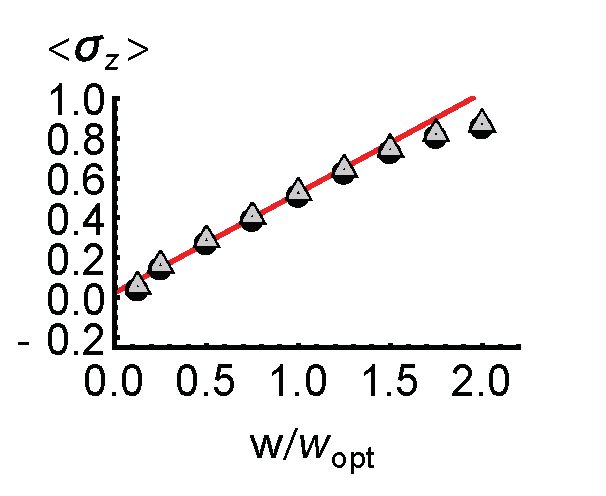
\includegraphics[scale =0.38] {N40SuperradianceSZ.eps}
	\hspace{-5.0mm} 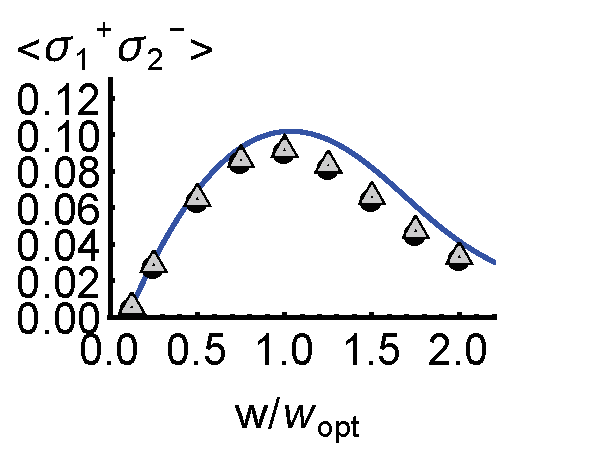
\includegraphics[scale =0.38] {N40SuperradianceSPSM.eps}
	\hspace{-5.0mm} 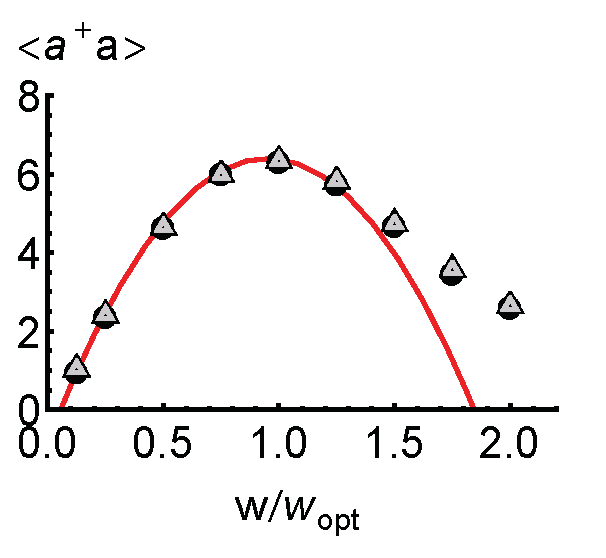
\includegraphics[scale =0.38] {N40Superradianceada.eps}
	\hspace{-5.0mm} 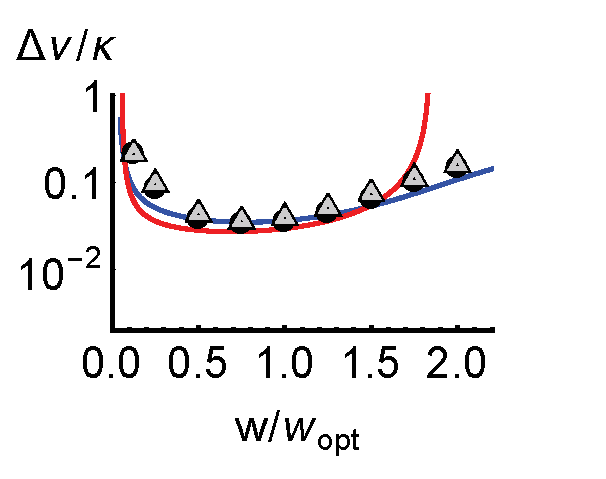
\includegraphics[scale =0.38] {N40SuperradianceLW.eps}
	\hspace{-5.0mm} 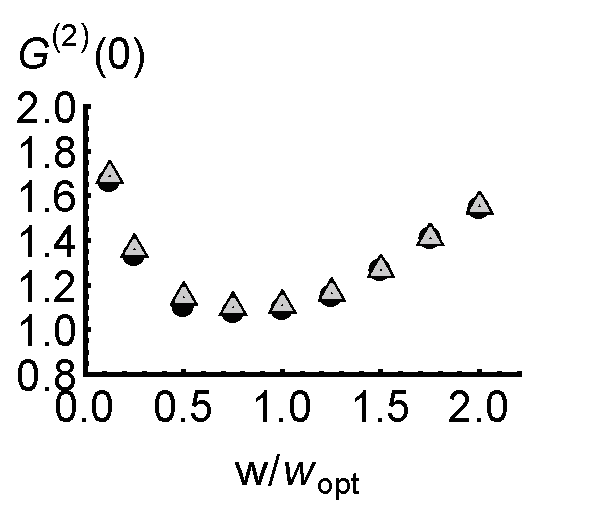
\includegraphics[scale =0.38] {N40SuperradianceG2.eps}\\ \vspace{0mm}
	\rotatebox{90}{ \hspace{7mm} \textbf{Crossover}}
	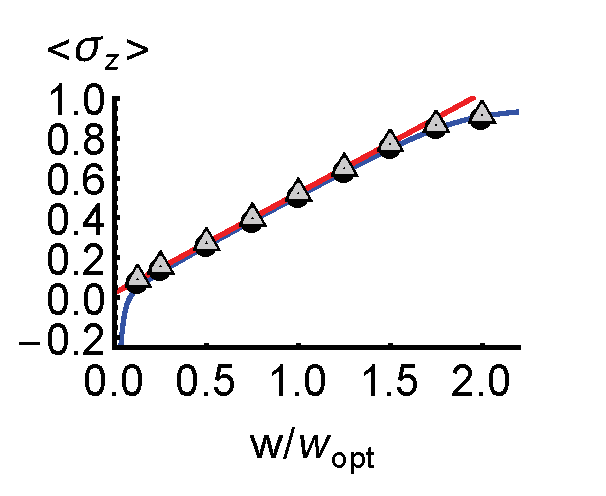
\includegraphics[scale =0.38] {N40CrossoverSZ.eps}
	\hspace{-5.0mm} 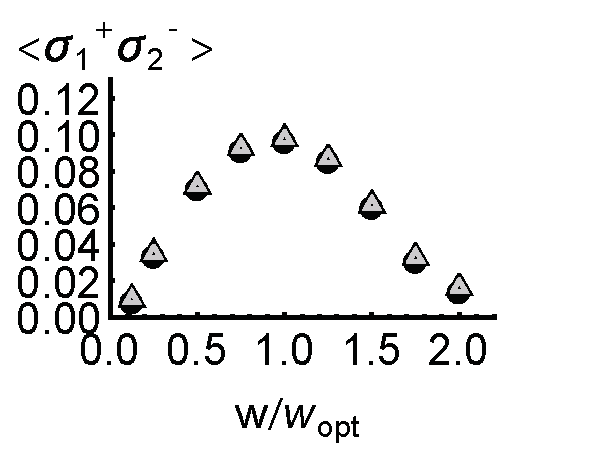
\includegraphics[scale =0.38] {N40CrossoverSPSM.eps}
	\hspace{-5.0mm} 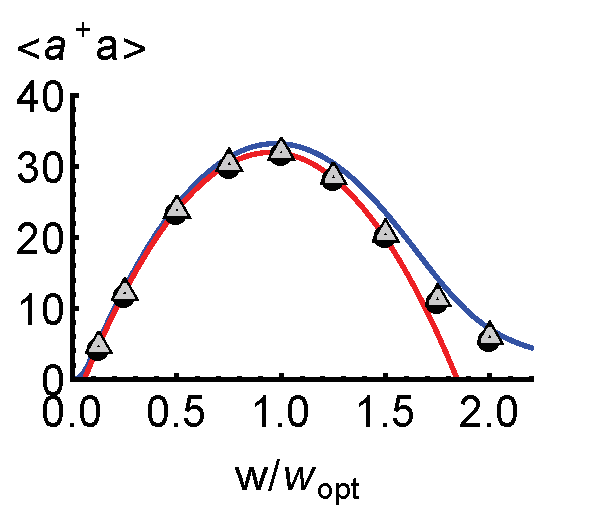
\includegraphics[scale =0.38] {N40Crossoverada.eps}
	\hspace{-5.0mm} 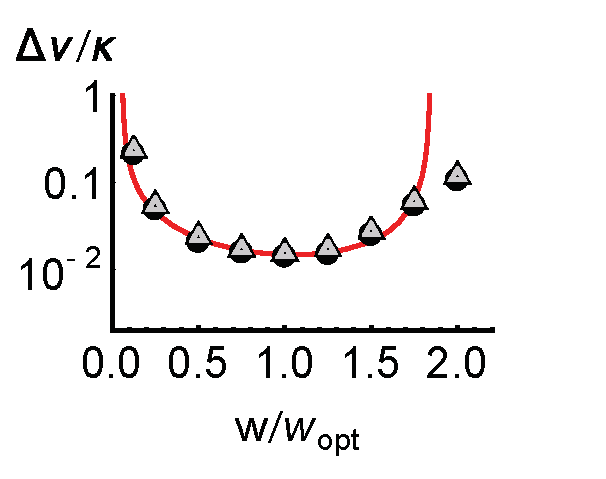
\includegraphics[scale =0.38] {N40CrossoverLW.eps}
	\hspace{-5.0mm} 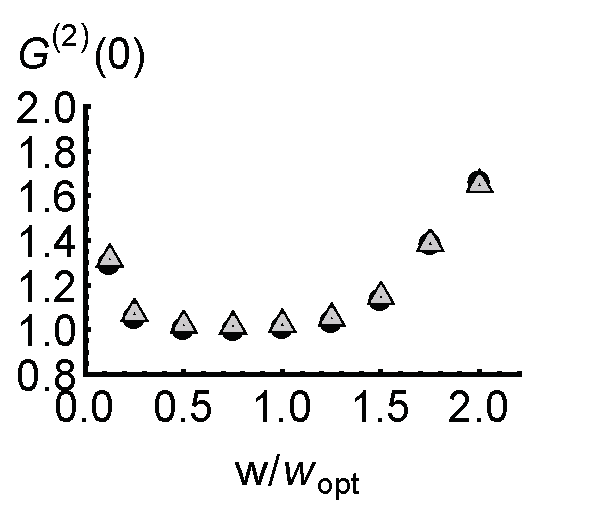
\includegraphics[scale =0.38] {N40CrossoverG2.eps}\\ \vspace{0mm}
	\rotatebox{90}{ \hspace{10mm} \textbf{Lasing}}
	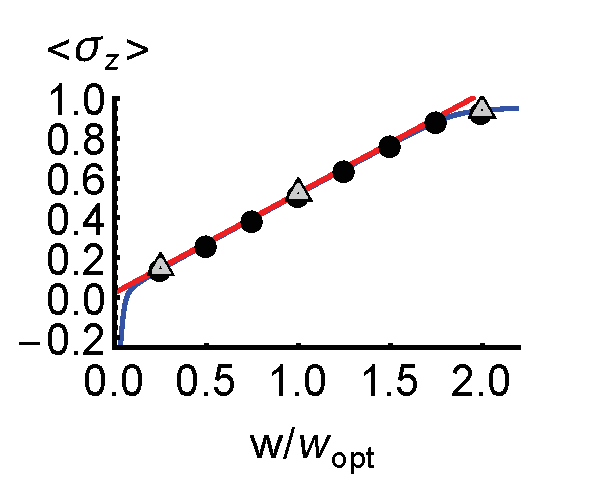
\includegraphics[scale =0.38] {N40LaserSZ.eps}
	\hspace{-5.0mm} 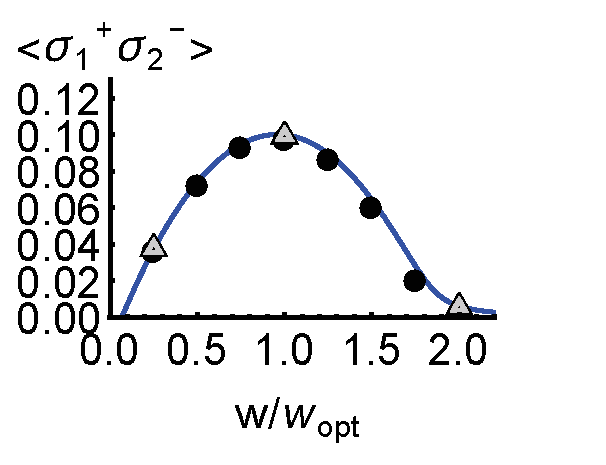
\includegraphics[scale =0.38] {N40LaserSPSM.eps}
	\hspace{-5.0mm} 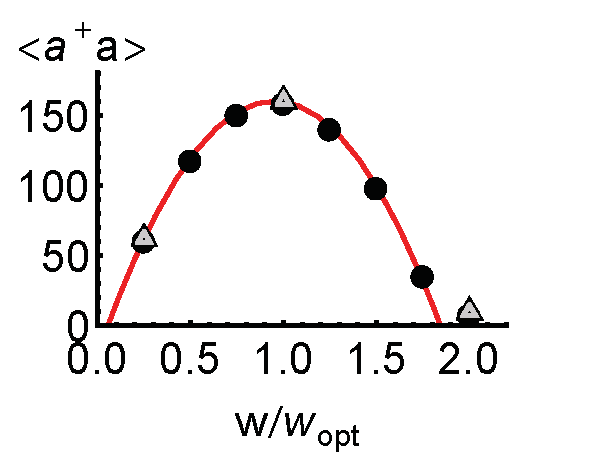
\includegraphics[scale =0.38] {N40Laserada.eps}
	\hspace{-5.0mm} 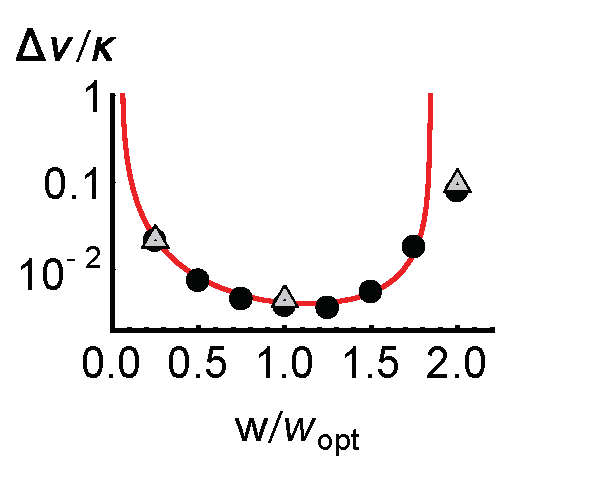
\includegraphics[scale =0.38] {N40LaserLW.eps}
	\hspace{-5.0mm} 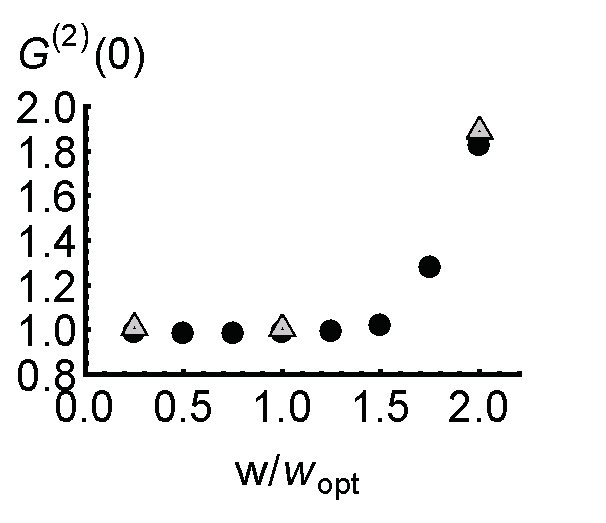
\includegraphics[scale =0.38] {N40LaserG2.eps}\\ \vspace{1mm}
	\hspace{5mm}(a)\hspace{30mm}(b) \hspace{30mm}(c) \hspace{30mm}(d) \hspace{30mm}(e)
\end{center}
		\vspace{-5mm}
\caption{(Color online) Comparison of the different solution methods in
the superradiance ($\xi=0.2$), crossover ($\xi=1$), and lasing ($\xi=5$)
regions for $N=40$ and $\frac{\Omega^2}{\kappa \gamma}=1$.  The analytic
Langevin (phase diffusion and mean field) solutions are shown in red
(light gray), the exact SU(4) solution is shown by grey triangles, and the {\it
c}-number Langevin simulation results are shown by black circles. The
observables considered are (a) the inversion
$\left<\hat{\sigma}^{z}\right>$, (b) the correlation between the atoms'
dipoles $\left<\hat{\sigma}_{1}^{+} \hat{\sigma}_{2}^{-}\right>$, (c)
the intracavity photon number  $\left<\hat{a}^{\dagger}\hat{a}\right>$,
(d) the linewidth $\Delta \nu$, and (e) the intensity correlation
function $G^{(2)}(0)$.}
\label{N40Comparison}
\end{figure*}


\section{Characterization of the Crossover}
\label{sec:CrossoverCharacterization}

The crossover from superradiance to lasing is characterized by a
transition from coherence stored in an atomic ensemble to coherence
stored in the light field. The key parameter in identifying the regime
is the ratio of the number of photons to the number of atoms when the
system is operated at its most efficient point in terms of output
intensity and spectral frequency width. With this motivation, we
introduce a crossover parameter as
\begin{equation}
\xi \equiv \frac{(|a_0|^2)_{opt}}{N},
\label{crossoverparam}
\end{equation}
that is, the dimensionless ratio of the intracavity photon number to
the number of atoms. The parameter $\xi$ quantifies the relative
importance of stimulated emission to collective atomic spontaneous
emission. If $\xi\ll1$, the system is in the bad cavity or
superradiant regime. If $\xi\gg1$ the system is in the good cavity or
laser regime. In the crossover or intermediate region, $\xi\sim1$, and
the system possesses features of both.

The mean field equations allow us to rewrite this expression in an
alternate way the illuminates the role of the system parameters in
determining the operating regime. From Eq.~(\ref{adaopt}), which is
applicable when the optimal repump rate $w_{\rm opt}$ is much larger
than the single atom decay $\gamma$ and dephasing $1/T_2$,
Eq.~(\ref{crossoverparam}) can be rewritten as an approximately
equivalent definition
\begin{equation}
\xi\approx \frac{N \Omega^2}{8\kappa^2}\;.
\label{CrossoverParameter2}
\end{equation}
The interpretation of this is that the crossover is also characterized
by the ratio of the collective coupling between the many atom ensemble
and the cavity mode, {\em i.e.}\ $N\Omega^2$, to the cavity mode decay
rate $\kappa$.

\section{Results}
\label{sec:Results}

In this section we present numerical results for field intensity,
inversion, line widths, and correlations throughout the crossover from
lasing to superradiance.  We begin by considering the different solution
methods for small numbers of atoms were we can compare with the exact
SU(4) Monte-Carlo results.  This comparison shows that the semi-classical
theory gives an accurate description of first and second moments of the
system operators.  This is an interesting result in itself besides
verifying the semi-classical methods because it demonstrates that the
system is not strongly correlated and we don't need to account for
genuinely quantum fluctuations.

With the validity of the semi-classical method established we then
consider systems with large numbers of atoms.  These systems are
experimentally relevant and allow us to more clearly understand the
behavior of the system in the large $N$ limit.

For simplicity, in all of these simulation results, we consider the
parameter regime in which the single atom rates $\gamma$ and $1/T_2$
are negligible compared to the cavity loss rate $\kappa$ and use
Eq.~(\ref{CrossoverParameter2}) to define $\xi$.

\begin{figure*}
\begin{center}
	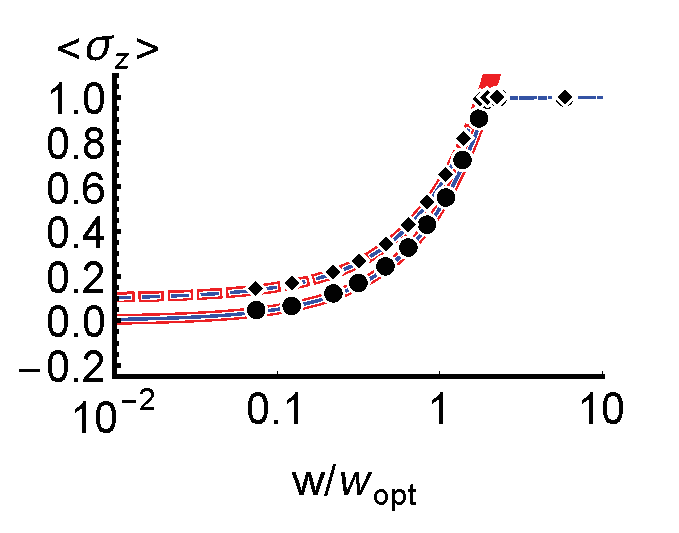
\includegraphics[scale =0.445] {N10000SZ.eps}
	\hspace{-5.0mm} 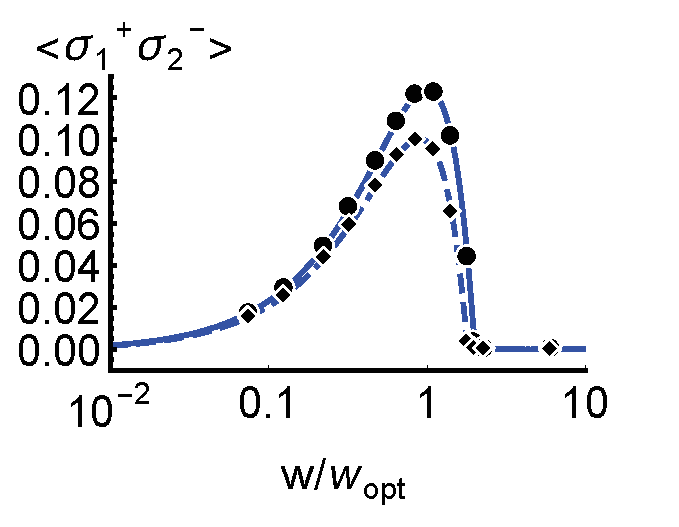
\includegraphics[scale =0.445] {N10000SPSM.eps}
	\hspace{-6.5mm} 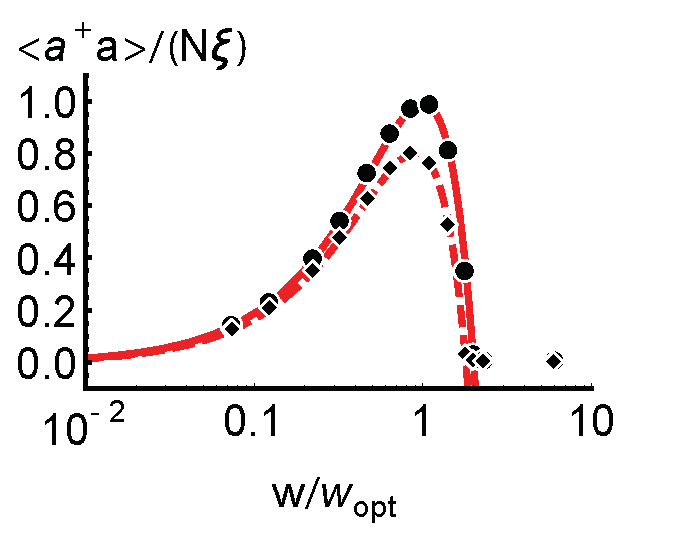
\includegraphics[scale =0.445] {N10000ada.eps}
	\hspace{-5.5mm} 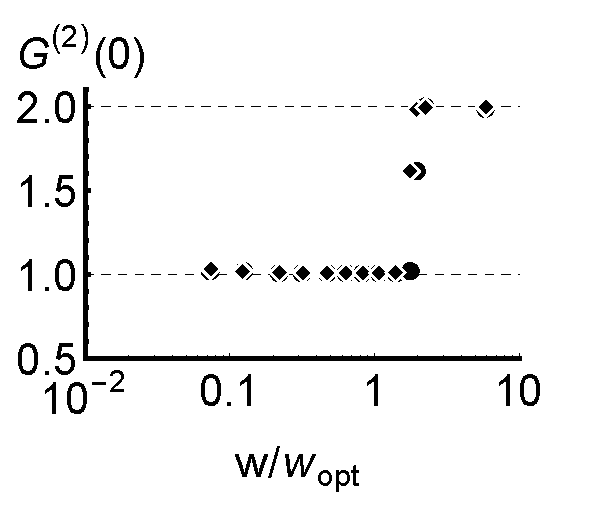
\includegraphics[scale =0.445] {N10000G2S.eps}\\
	\textbf{(a) Universal}\\
	\line(1,0){500}\\
	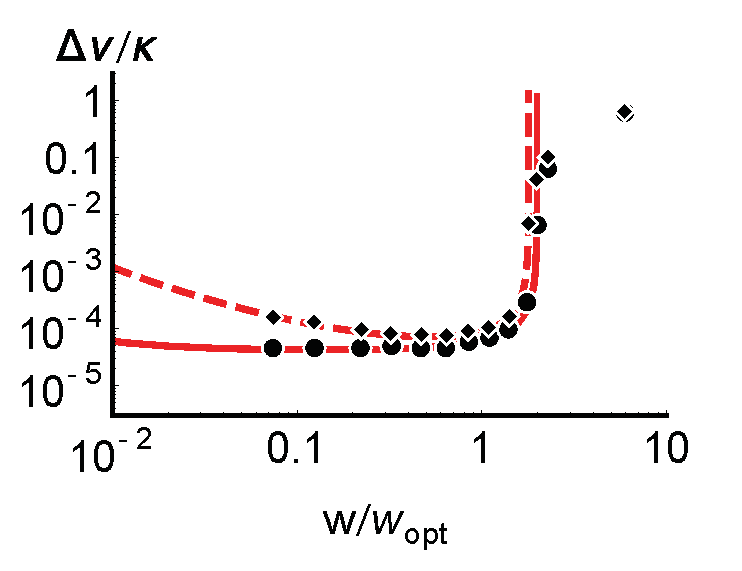
\includegraphics[scale =0.51] {N10000LWS.eps}
	\hspace{-5.5mm} 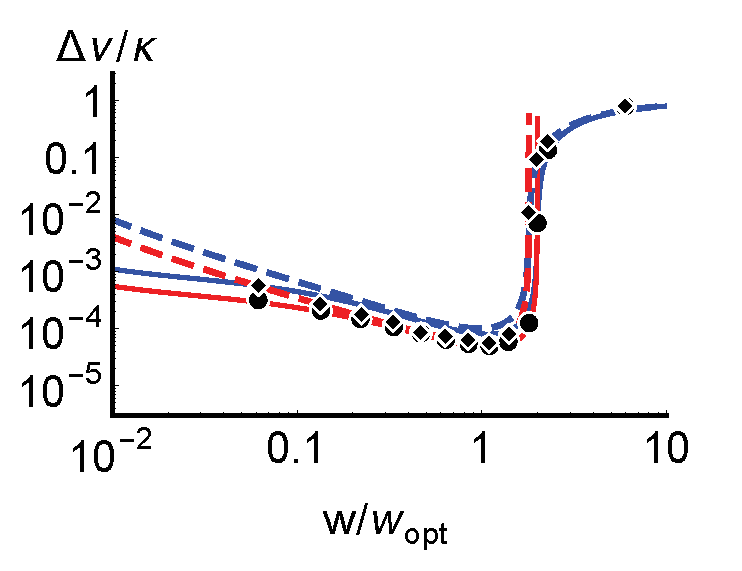
\includegraphics[scale =0.51] {N10000LWC.eps}
	\hspace{-5.5mm} 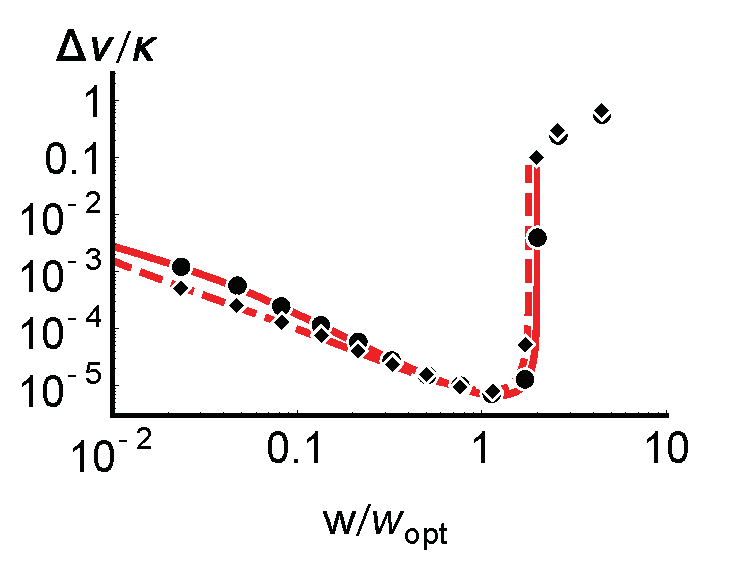
\includegraphics[scale =0.51] {N10000LWL.eps}\\
	\hspace{-10mm}\textbf{(b) Superradiance}\hspace{33mm}\textbf{(c) Crossover}
  \hspace{37mm}\textbf{(d) Lasing}
\end{center}
		\vspace{-5mm}
\caption{(Color online) Solutions using the various methods in the
superradiance ($\xi=0.1$), crossover ($\xi=1$), and lasing ($\xi=10$)
regions for N=10000 and $\frac{\Omega^2}{\kappa \gamma}=0.1$. For
$1/T_2=0$, the analytic Langevin (phase diffusion and mean field)
solutions are shown in solid red (solid light gray), and the
{\it c}-number Langevin simulation results are shown by black circles.
For $1/T_2=\frac{1}{5} w_{opt}$, the analytic Langevin solutions are
shown in dashed red (dashed light gray), and the {\it
c}-number Langevin simulation results are shown by black diamonds. (a)
All observables considered except linewidth  $\Delta \nu$ show universal
behavior in the superradiance, crossover, and lasing regions, after
appropriate scaling.  (b)  $\Delta \nu / \kappa$ in the superradiance
region (c) $\Delta \nu / \kappa$ in the crossover region, (d) $\Delta
\nu / \kappa$ in the lasing region.}
 \label{N10000Comparison}
\end{figure*}


\subsection{Simulations with small atom numbers}

In order to determine the validity of the approximate solution methods,
we begin by comparing them to the exact solutions.  We use $N=40$ atoms
for the comparison.  This is a small enough to still be tractable by
exact SU(4) Monte-Carlo simulations and at the same time it is large
enough to expect the approximate solution methods to be reasonably
accurate. 

Specifically, Fig.~\ref{N40Comparison} shows several observables
obtained using the mean field Langevin method, the phase diffusion
method, the {\it c}-number Langevin method, and exact SU(4)
Monte-Carlo simulations for three different values of the crossover parameter:
$\xi=0.2$, $\xi=1$, and $\xi=5$. These values of $\xi$ put the system in the
superradiance, crossover, and lasing parameter regions, respectively.
We note that the SU(4) method becomes more computationally intensive as $\xi$ is increased, since there are more photons as $\xi$ is increased, and hence
more basis states need to be tracked. Therefore, for $\xi=5$, we used a
method that combines the SU(4) approach with the quantum jump method (see Appendix~\ref{Su4Appendix}).

Fig.~\ref{N40Comparison} shows excellent agreement between {\it
c}-number Langevin and the exact SU(4) theory in all parameter regions
for all of the considered observables. Therefore, the {\it c}-number
Langevin theory can be relied upon for larger atom numbers inaccessible
to direct numerical simulation.

Figures~\ref{N40Comparison} (a) and (c) show that the mean field
equations are accurate near the collective emission peak, $w/w_{opt}=1$,
but they are less accurate outside that region.
Figure~\ref{N40Comparison} (d), shows that the phase diffusion model for
the linewidth also agrees in the region around $w/w_{opt}=1$, but
disagrees outside that region, where the phase diffusion approximation
breaks down.  Although they do not quantitatively agree with the exact
SU(4) method, the analytic solutions obtained by the mean field and
phase diffusion models capture the correct qualitative behavior of the
system.


\subsection{Simulations with large atom numbers}

Now that an agreement between the {\it c}-number Langevin and exact
SU(4) theories has been established, we study more experimentally
realistic systems with $N=10000$ using the semi-classical theory based
on the {\it c}-number Langevin equations. We also include the mean field
Langevin theory, the phase diffusion model for the linewidth. The
results of these simulations are shown in Fig.~\ref{N10000Comparison}.
We consider both the case of vanishing inhomogeneous broadening,
$1/T_2=0$, as well as $1/T_2=w_{opt}/5$.

As seen in Fig.~\ref{N10000Comparison} (a), when $1/T_2=0$, the
inversion $\left<\hat{\sigma}^{z}\right>$, the correlation between atoms
$\left<\hat{\sigma}_{1}^{+} \hat{\sigma}_{2}^{-}\right>$, the
intracavity photon number  $\left<\hat{a}^{\dagger}\hat{a}\right>$,  and
the intensity correlation function $G^{(2)}(0)$ all show universal
behavior in the superradiance, crossover, and lasing regimes after
appropriate scaling.  For $1/T_2=w_{opt}/5$ these observables still show
universal behavior after appropriate scaling, and the values do not
change significantly from the $1/T_2=0$ case.

It is worth noting that, even though  $\left<\hat{\sigma}_{1}^{+}
\hat{\sigma}_{2}^{-}\right>$ has universal behavior throughout the
crossover, typical lasers operate just above threshold in terms of the
scaled quantities, i.e. $w \ll w_{opt}$.  Just above threshold the
atom-atom correlations are typically very small,
\begin{equation}
\left<\hat{\sigma}_{1}^{+}\hat{\sigma}_{2}^{-}\right>_{opt} \ll 1\;.
\end{equation}
Thus atom-atom correlations are usually not important in lasers.

The linewidth $\Delta \nu$, however, does not show universal behavior in
the superradiance, crossover, and lasing regimes. As seen in
Fig.~\ref{N10000Comparison} (b), in the superradiance region, when
$1/T_2=0$, $\Delta \nu / \kappa$ is flat in the region of $w/w_{opt}<1$.
In contrast, the linewidth in the lasing regime, shown in
Fig.\ref{N10000Comparison} (d), linearly decreases as $w/w_{opt}$
increases towards unity. This is the typical Schawlow-Townes behavior,
which can be seen by considering
$\kappa/\left<\hat{a}^{\dagger}\hat{a}\right>$ using Eq.~\ref{a0sqSS}.
In the crossover region, shown in Fig.~\ref{N10000Comparison} (c), we
see that for $w/w_{opt}\ll 1$ , $\Delta \nu/\kappa$ is flat, and as
$w/w_{opt}$ approaches unity, $\Delta \nu/\kappa$ starts to linearly
decrease as in the lasing regime. Therefore, a system in the crossover
region displays characteristics of both superradiance and lasing. 

When $1/T_2$ is increased to $1/T_2=w_{opt}/5$,
Fig.~\ref{N10000Comparison} (b) shows that $\Delta \nu/\kappa$ increases
for $w/w_{opt}\ll 1$, but it is not significantly affected by $1/T_2$ as
$w/w_{opt}$ approaches unity.  Note that the latter is the pumping
region where the emitted light intensity is largest.  Near $w\sim w_{\rm
opt}$ we obtain both the largest intensity and the best frequency
stability.

In the crossover region, seen in Fig.~\ref{N10000Comparison} (c), when
$1/T_2=w_{opt}/5$, $\Delta \nu/\kappa$ increase for $w/w_{opt}\ll 1$,
where the system is displaying superradiant behavior.  On the other
hand, when $w \sim w_{opt}$ where the
system starts to display lasing behavior, $\Delta\nu/\kappa$ is
insensitive to the inhomogeneous broadening of the atomic line.

Figure~\ref{N10000Comparison} (d) shows that $\Delta \nu/\kappa$ does
not increase in the lasing region when $1/T_2=w_{opt}/5$.  Rather the
linewidth decrease in the region slightly below $w/w_{opt}=1$, when
compared to the $1/T_2=0$ case. This reduction has also been observed
for smaller atom numbers using the exact SU(4) code. It can be shown
that the value of $1/T_2$ that maximally reduces the linewidth is
$1/T_2=\frac{w_{opt}}{1+\sqrt{2}}$.
\dmcomment{Do we have an intuitive explanation of this result? DT Answer: I do not have an intuitive understanding of this result. I included it just incase it sparked the interest of someone else.}

As mentioned previous, a laser normally operates just above threshold,
where $w/w_{opt} \ll 1$. As seen in Fig.~\ref{LWadaComparison} (a), for
the same pump strength $w$, and a fixed $N$, a system in the crossover
region can operate with $w/w_{opt} = 1$, allowing the crossover system
to have a linewidth orders of magnitude smaller than the linewidth of
the lasing system.  Fig.~\ref{LWadaComparison} (b) shows that this
improvement in linewidth can be achieved without paying the penalty of a
reduced output intensity.  Another way of saying this is that, for the
same output intensity, one can achieve greater brightness of the light
source by using atoms with a smaller linewidth.


\subsection{Effect of Cavity and Atomic Level Instabilities on the
Spectrum}

The effect of instabilities in the cavity frequency and atomic frequency
on the linewidth is now investigated. Cavity frequency instability can
be caused by fluctuations in cavity length due to the thermal
fluctuations of the cavity mirrors, which are unavoidable in an
experiment. The energy levels in an atom can also be shifted by stray
electromagnetic fields. The frequency of the combined atom-cavity system
$\omega$ lies somewhere between the bare atom and cavity frequencies,
and is given by Eq.~(\ref{atomcavityfrequencycenter1}).

\begin{figure}
\begin{center}
	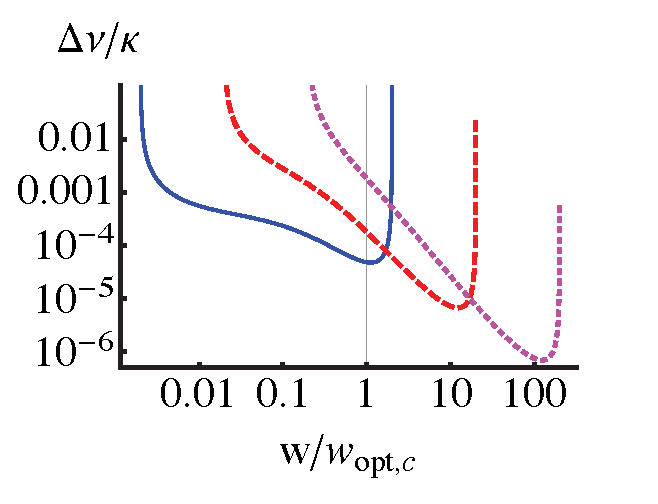
\includegraphics[scale =0.415] {LinewidthComparisonLangevin.eps}
	\hspace{-4mm} 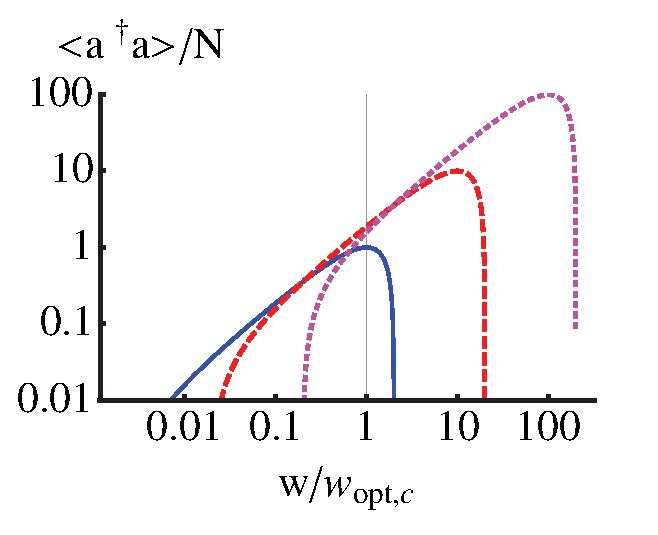
\includegraphics[scale =0.415] {adaComparisonLangevin.eps}\\
	\hspace{6mm}\textbf{(a)}\hspace{37mm}\textbf{(b)} \hspace{35mm}
\end{center}
		\vspace{-5mm}
\caption{(Color online) Comparison of (a) linewidth and (b) intra-cavity
intensity for a system in the crossover ($\xi=1$) shown in blue solid,
lasing ($\xi=10$) shown in red dashed, and far lasing ($\xi=100$) shown
in magenta dotted, regions using the analytic (phase diffusion and mean
field) Langevin model. $w_{opt,c}$ is the optimum $w$ value in the
crossover region. For all systems, $N=10000$ and $\frac{\Omega^2}{\kappa
\gamma}=0.1$.}
\label{LWadaComparison}
\end{figure}

If $\omega$ is varied, the resultant time averaged linewidth will be an
average over these values, and will hence be much broader than the
quantum limited linewidth. Therefore, the derivative of  $\omega$ with
respect to $\omega_c$, and with respect to $\omega_a$, gives us an idea
as to how much of an effect an instability in these frequencies will
have on broadening the linewidth. These derivatives are plotted in
Fig.~\ref{CavityInstability}.

Fig.~\ref{CavityInstability} (a) tells us that on the lasing side of the
crossover, $\omega$ is shifted proportionally to the shift in
$\omega_c$, while on the superradiant side, $\omega$ is insensitive to
shifts in $\omega_c$.  Conversely, in Fig.~\ref{CavityInstability} (b)
it can be seen $\omega$ is shifted proportionally to the shift in
$\omega_a$ on the superradiance side of the crossover, while on the
lasing side, $\omega$ is insensitive to shifts in $\omega_a$. In the
intermediate regime ($\xi=1$), $\omega$ is not as sensitive to a shift
in the $\omega_c$ as it is in the laser regime, and it is not as
sensitive to a shift in the $\omega_a$, as it is on the superradiance
side.

\section{Conclusion}

A model that is capable of describing a system operating in any
parameter region of the crossover between steady state superradiance and
lasing was introduced. Since this model can only be solved exactly for small systems, several solution methods that treat the quantum fluctuations with varying degree of approximation were introduced, based on the property that in these systems, fluctuations scale inversely with the number of particles.  First, mean field equations, which neglect all quantum fluctuations, were used to derive analytic expressions for many of the system observables. These analytic expressions were used to motivate the definition of the crossover parameter. Since the mean field equations cannot describe the spectral properties of the system, the method {\it c}-number Langevin equations with Gaussian fluctuations was introduced. For small systems, where the exact SU(4) method can be applied, the {\it c}-number Langevin method showed excellent agreement with the exact SU(4) method. Therefore, the {\it c}-number Langevin method was used to treat larger systems, and a comparison of the properties of systems operating in the different parameter regions of the crossover was made. 

\begin{figure}
\begin{center}
	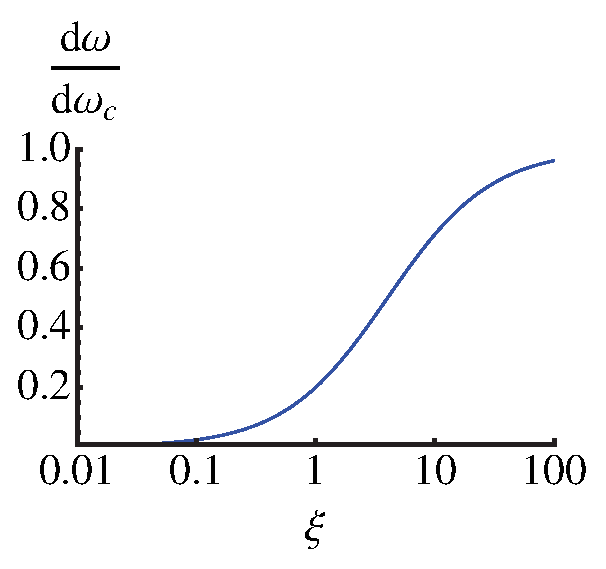
\includegraphics[scale=0.42] {CavityInstability.eps} \hspace{2mm}
	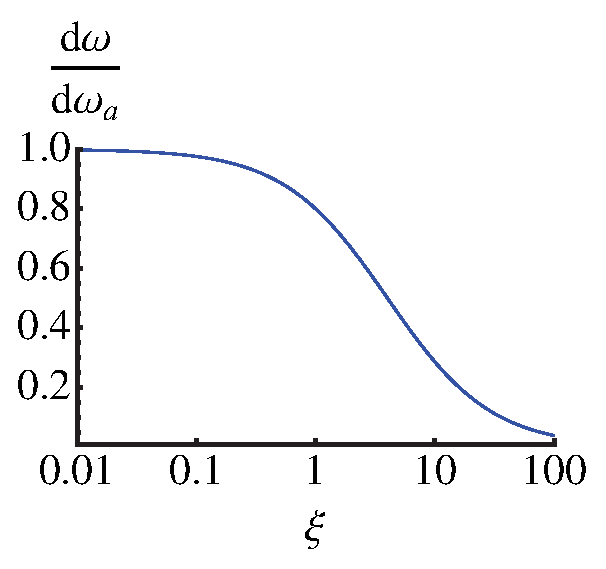
\includegraphics[scale=0.42] {AtomInstability.eps}\\
\hspace{2mm} \textbf{(a)}\hspace{40mm}\textbf{(b)} \hspace{35mm}
\end{center}
\caption{(Color online) Instability in the atom-cavity system frequency
$\omega$ with respect to (a) the cavity frequency $\omega_c$ and (b)
atomic frequency $\omega_a$ as a function of crossover parameter $\xi$. These results were calculated using Eq.~(\ref{atomcavityfrequencycenter1}).}
\label{CavityInstability}
\end{figure}

Although a system in the lasing parameter region is capable of
possessing the smallest linewidth, typically lasers operate with a
re-pumping rate that puts them just above threshold, which does not
allow the smallest linewidth for the system to be realized. For the same
re-pumping rate, a system operating in the crossover region will be
farther above threshold, potentially allowing for a linewidth orders of
magnitude smaller than in the laser region. Also, a crossover system
will have a larger intracavity intensity than a superradiant system,
making the former more experimentally accessible.

It was also demonstrated that a system in all regions of the crossover
is insensitive to atomic dephasing as long as the re-pumping rate is
smaller than the dephasing rate. Also, as the crossover is traversed
into the lasing region, atomic dephasing can actually cause a reduction
in the linewidth.

Finally, it was shown that the linewidth on the superradiance side is
insensitive to fluctuations in cavity length, and that these
fluctuations become more important as the crossover is traversed toward
the laser side. Conversely, it was shown that the linewidth on the
lasing side is insensitive to fluctuations in the atomic energy levels,
and that these fluctuations become more important on the superradiance
side. A system in the crossover region will be less sensitive to cavity
frequency fluctuations than a lasing system, and it will be less
sensitive to atomic frequency instabilities than a superradiant system.
Both of these fluctuations cause a broadening of the linewidth. These
conclusions are significant since fluctuations in the cavity frequency
are a principal limitation preventing further reduction of the linewidth
in today's most ultrastable lasers.

This work has been supported by JILA-NSF-PFC-1125844, DARPA, QuASAR, and
NIST.

\appendix

\section{SU(4) Numerical Simulation of the Master Equation}
\label{Su4Appendix}

Recently, we have developed a group-theoretic method for efficiently
simulating the quantum master equation~\cite{PhysRevA.87.062101}. In brief, the
master equation, Eq.~(\ref{ME1Crossover}), can be expressed in terms of
generators of the SU(4) group, with the Hamiltonian part being,
\begin{eqnarray}
  &&\frac{1}{i\hbar}[H,\rho]=
  -2i \omega_a \Sigma_3\rho -i\omega_c [ \hat{a}^{\dagger}\hat{a}, \rho]
  \nonumber
  \\
  &&-i\Omega \left[a(\mathcal{M}_++\mathcal{N}_+)\rho+a^\dagger
    (\mathcal{M}_-+\mathcal{N}_-)\rho\right]\nonumber\\
  &&\quad{}+i\Omega\left[(\mathcal{U}_++\mathcal{V}_+)\rho a^\dagger
    +(\mathcal{U}_-+\mathcal{V}_-)\rho a\right]\,,
\end{eqnarray}
and dissipation parts being,
\begin{eqnarray}\label{liv}
 && \sum_{j=1}^N(
   2\sigma_j^-\rho\sigma_j^+-\sigma_j^+ \sigma_j^-\rho-
   \rho \sigma_j^+\sigma_j^-
  )/2=-\frac{N}{2}-
  \mathcal{Q}_3+\mathcal{Q}_{-}\,,\nonumber\\
 && \sum_{j=1}^N(
   2\sigma_j^+\rho\sigma_j^--\sigma_j^- \sigma_j^+\rho-
   \rho \sigma_j^-\sigma_j^+
  )/2=-\frac{N}{2}+
  \mathcal{Q}_3+\mathcal{Q}_{+}\,,\nonumber\\
 && \sum_{j=1}^N(\sigma_j^{(3)}\rho\sigma_j^{(3)}-\rho)=4\mathcal{M}_3-2
  \mathcal{Q}_3-2\Sigma_3-N\,,
  \label{ham}
\end{eqnarray}
where $\mathcal{Q}_{\pm}$, $\mathcal{M}_{\pm}$, $\mathcal{N}_{\pm}$,
$\mathcal{U}_{\pm}$, $\mathcal{V}_{\pm}$, $\mathcal{Q}_3$, $\mathcal{M}_3$,
and $\Sigma_3$ are superoperators~\cite{PhysRevA.87.062101}.  As a result, we can
expand the density matrix in terms of the fully symmetrical multiplet
$P_{q,q_3,\sigma_3}$~\cite{PhysRevA.87.062101} of the SU(4) group,
\begin{equation}\label{ex}
  \rho=\sum_{q,q_3,\sigma_3,m,n} C_{q,q_3,\sigma_3}^{m,n}
  P_{q,q_3,\sigma_3}\bigl|m\bigr>\bigl<n\bigr|\,,
\end{equation}
where $C_{q,q_3,\sigma_3}^{m,n}$ are complex coefficients, and
$|n\rangle$ is the photon Fock state. Note that the total number of
states in the fully symmetrical multiplet is $1/6 (N+1)(N+2)(N+3)$,
which reduces the exponential scaling of the problem to cubic in $N$.
This has enabled us to numerically investigate large
systems~\cite{PhysRevA.87.062101}.

However, the number of basis in Eq.~(\ref{ex}) also grows as square of
the photon number.  This would impose great difficulties in numerical
simulations of the laser region due to the large number of photons.
Below, we present a method that unravels the master equation in the
Liouville space, which enables us to remove the photon basis in the
simulation. The essential idea behind the method is that we are able to
deduce the photon state by keeping track of the total number of quanta
$N_q$ in the system.

The quantum Monte Carlo method decomposes the density operator evolution
into a set of quantum trajectories where, between applications of random
jumps into random channels, the system evolves under an effective
Hamiltonian~\cite{Dalibard92,Dum92,Knight98}. These random jumps are chosen with the proper weights, so that when many trajectories are averaged over, the correct density operator evolution is given. While this has
conventionally been done with wavefunctions to reduce the numerical
complexity, here we apply the quantum trajectory algorithm in the
density matrix space in order to get rid of the photon basis in the
expansion of the density operator. To construct a single trajectory, we
first need to identify the jump operators. In our problem, there are
four decay channels: repumping, spontaneous emission, dephasing and
cavity decay. The corresponding jump operators $\mathcal{J}_i$ are
\begin{eqnarray}
\mathcal{J}_1\rho&=&
w\sum_{j=1}^N(\sigma_j^+\rho\sigma_j^-)=w\mathcal{Q}_{+}\rho\,,
\nonumber\\
\mathcal{J}_2\rho&=&
\gamma\sum_{j=1}^N(\sigma_j^-\rho\sigma_j^+)=
\gamma \mathcal{Q}_{-}\rho\,,\nonumber\\
\mathcal{J}_3\rho&=&
\frac{1}{2T_2}\sum_{j=1}^N(\sigma_j^{(3)}\rho\sigma_j^{(3)})
\nonumber\\
&=&\frac{1}{2T_2}(4\mathcal{M}_3-2  \mathcal{Q}_3-2\Sigma_3)\rho\,,
\nonumber\\
\mathcal{J}_4\rho&=&\kappa a\rho a^{\dagger}\,.
\label{jumpo}
\end{eqnarray}
When a repumping quantum jump happens, $N_q$ is decreased by one. When a
spontaneous emission or a cavity-decay quantum jump happens, $N_q$ is
increased by one. The dephasing quantum jump also does not change the
total number of quanta. Therefore, during the evolution of a single
trajectory, one could calculate $N_q$ at every time step by tracking the
the numbers of jumps of the different types. With the knowledge of
$N_q$, the photon state can be easily deduced. It is shown in
Ref.~\cite{PhysRevA.87.062101} that
\begin{equation}
\begin{split}
  \hat{J}_3P_{q,q_3,\sigma_3}^{(\mathrm{s})}&=
  (q_3+\sigma_3)P_{q,q_3,\sigma_3}^{(\mathrm{s})},\\
  P_{q,q_3,\sigma_3}^{(\mathrm{s})}\hat{J}_3&=
  (q_3-\sigma_3)P_{q,q_3,\sigma_3}^{(\mathrm{s})},
\end{split}
\end{equation}
where $\hat{J}_3=\sum_{j=1}^N\sigma_j^{(3)}/2$ is the collective spin
operator. Therefore, the atomic state for a particular fully symmetrical
atomic basis in terms of the number of excited atoms is
$|q_3+\sigma_3+N/2\rangle\langle q_3-\sigma_3+N/2|$. And thus the
corresponding photon state is
\begin{equation}
\bigl|m\bigr>\bigl<n\bigr|=
\bigl|N_q-(q_3+\sigma_3+N/2)\bigr>
\bigl<N_q-(q_3-\sigma_3+N/2)\bigr|.
\end{equation}
Therefore, if the system starts in a photon number state, by counting the quantum jumps, we have complete knowledge of
photon states for every single trajectory. This enables us to remove the
photon basis, which greatly improves the efficiency of the method. 

The simulation of jump times and jump channels is completely analogous
to the wave-function Monte Carlo method. The effective evolution of the
system is governed by the master equation excluding the above jump
operators. As a result, under the effective evolution, the trace of the
density operator is no longer conserved, but decreases as a function of
time.  This is analogous to the decay of the norm of the wavefunction in
the wave function Monte Carlo method. A jump occurs when the trace of
the density operator is less than a random number uniformly distributed
in the interval $[0,1]$. When a decay occurs we stochastically determine
the channel $i$ into which the system decays according to the
probability distribution,
\begin{equation}
\mathcal{P}_i^{\mathrm{jump}}=\frac{\mathrm{Tr}[\mathcal{J}_i\rho]}{\sum_{k=1}^4
\mathrm{Tr}[\mathcal{J}_k\rho]}.
\end{equation}

Finally, in order to get the density operator at each time step, an
ensemble average of many quantum trajectories is required. Then, various
observables can be calculated according to Ref.~\cite{PhysRevA.87.062101}. It is
also worth noting that if one is only interested in the steady state
density operator, a time average in the steady state can be applied
instead of the ensemble average.

\section{Phase Diffusion Linewidth}
\label{HakenAppendix}

The linewidth due to the phase fluctuations of $\hat{a}$ is derived from the quantum Langevin equations, Eqns.~(\ref{La})~--~(\ref{Lsz}). Following closely to the derivation done in \cite{HakenLaser,
HakenLaserBook}, Eq.~(\ref{La}) is differentiated, and substituted into
it Eqns.~(\ref{La})~--~(\ref{Lsm}) and the integral of Eq.~(\ref{Lsz}), to
arrive at an equation for $\hat{a}$ alone,
\begin{equation}
\ddot{\hat{a}} =
-\frac{1}{2} (\kappa+\Gamma)  \dot{\hat{a}} -
\frac{\kappa \Gamma}{4}\hat{a}  +
\frac{N \Omega^2 }{4} \hat{a} \hat{S}^z +\hat{F},
\label{addeq}
\end{equation}
where
\begin{eqnarray}
\hat{S}^z &=&
\int_0^t dt^{\prime} e^{-(w+\gamma)(t-t^{\prime})}
\bigg( (w+\gamma) + \hat{F}^z
\nonumber
\\
&&\hspace{-3mm}-\frac{2}{N} \left( \frac{d}{dt} (\hat{a}^{\dagger} \hat{a}) +
\kappa \hat{a}^{\dagger} \hat{a} -\hat{a}^{\dagger} \hat{F}^a -
\hat{F}^{a^{\dagger}} \hat{a} \right) \bigg),
\end{eqnarray}
and,
\begin{equation}
\hat{F} = \frac{\Gamma}{2} \hat{F}^a-
\frac{i N \Omega}{2} \hat{F}^-+\dot{\hat{F}}^a.
\end{equation}
The annihilation operator $\hat{a}$ is decomposed according to,
\begin{equation}
\hat{a}= (a_0 + \hat{\rho}) e^{i\hat{\phi}}.
\label{adecomp}
\end{equation}
Above threshold, amplitude fluctuations are expected to be small, so that
\begin{equation}
\left< \hat{a}^{\dagger}(t) \hat{a}(0) \right> =
a_0^2 \left< e^{i(\hat{\phi}(t) - \hat{\phi}(0))} \right>.
\end{equation}

After substituting Eq.~(\ref{adecomp}) into Eq.~(\ref{addeq}), we take
the imaginary part to first order in products of operators, and find,
\begin{equation}
\ddot{\hat{\phi}} =
-\frac{1}{2}(\kappa+\Gamma) \dot{\hat{\phi}} +
\frac{1}{a_0} \text{Im} [\hat{F}],
\label{phieq1}
\end{equation}
where a factor of $e^{-i\phi}$ has been absorbed into $\hat{F}$.
Eq.~(\ref{phieq1}) is then integrated, assuming that $(\kappa+\Gamma)$
is large, to arrive at,
\begin{equation}
\hat{\phi}(t) - \hat{\phi}(0) =
\frac{2}{a_0 (\kappa+\Gamma)}
\int_0^t dt^{\prime} \text{Im}
\left[ \frac{\Gamma}{2} \hat{F}^a-\frac{i N \Omega}{2} \hat{F}^-\right].
\label{phieq2}
\end{equation}
Since $ \hat{F}^a$ and $\hat{F}^-$ are Gaussian, we can use
\begin{equation}
\left< e^{i(\hat{\phi}(t) - \hat{\phi}(0))} \right> =
e^{-\frac{1}{2}\left< ( \hat{\phi}(t) - \hat{\phi}(0) )^2 \right>}.
\end{equation}
Therefore, we use Eq.~(\ref{phieq2}), along with Eqns.~(\ref{OpNoise1})
to find,
\begin{equation}
\left<(\hat{\phi}(t) - \hat{\phi}(0))^2 \right> =
\left(\frac{(C+1)}{2(Cd_0-1)} \frac{\Gamma}{(w+\gamma)}
\frac{\Omega^2 \kappa}{(\kappa+\Gamma)^2}\right) t,
\end{equation}
so that the linewidth $\Delta \nu$ given by,
\begin{equation}
\Delta \nu =
\frac{(C+1)}{2(Cd_0-1)} \frac{\Gamma}{(w+\gamma)}
\frac{\Omega^2 \kappa}{(\kappa+\Gamma)^2}.
\label{LWHaken}
\end{equation}

\bibliographystyle{unsrt}
\bibliography{CrossoverPaper}

\end{document}

% vim: nocindent spell
